\documentclass{beamer}

% ************ PACKAGES **************
\usepackage[utf8]{inputenc}
\usepackage{hyperref}
\usepackage[justification=centering]{caption}
\usepackage{graphicx}
% ************************************

% ************ TITLE DATA ************
\title{Particionado de Red Basado en Redes SDN}
\author{Autor: Ángel Guzmán Martínez \\[6pt] Tutor: Jorge Navarro Ortiz}
\institute{Departamento de Teoría de la Señal, Telemática y Comunicaciones \\[6pt] Universidad de Granada}
\titlegraphic{
\includegraphics[scale=0.25,trim={0 6.5cm 0 2cm},clip]{ugr_logo.png}}
\date{}
% ************************************

% ***** THEME AND TEMPLATE ***********
\usetheme{Warsaw}
%\usecolortheme{}
\setbeamertemplate{headline}{}
\setbeamertemplate{footline}[frame number]
\beamertemplatenavigationsymbolsempty
\setbeamerfont{page number in head/foot}{size=\large}
\setbeamerfont{institute}{size=\small, series=\bfseries}
% ************************************

\begin{document}

\begin{frame}
    \titlepage
\end{frame}

\begin{frame}{Índice}
    \begin{columns}[t]
        \begin{column}{1.7in}
            \tableofcontents[hideallsubsections, sections={1-4}]
        \end{column}
        \begin{column}{1.7in}
            \tableofcontents[hideallsubsections, sections={5-7}]
        \end{column}
    \end{columns}
\end{frame}

\section{Objetivos y Motivación}
\begin{frame}{Índice}
    \begin{columns}[t]
        \begin{column}{1.7in}
            \tableofcontents[currentsection, hideallsubsections, sections={1-4}]
        \end{column}
        \begin{column}{1.7in}
            \tableofcontents[currentsection, hideallsubsections, sections={5-7}]
        \end{column}
    \end{columns}
\end{frame}

\begin{frame}{Objetivos y Motivación}
    \textbf{Objetivos}\vspace{10pt}
    \begin{itemize}
        \item Entender las limitaciones de las redes tradicionales.
        \item Familiarizaros con el concepto de SDN y \textit{network slicing}.
        \item Particionar una red SDN y comprobar su funcionamiento.
    \end{itemize}\vspace{20pt}

    \onslide<2>{\textbf{¿Por qué particionar una red (\textit{network slicing})?}\vspace{10pt}
    \begin{itemize}
        \item Tráfico heterogéneo. IoT, eMBB, URLLC...
        \item Redes Tradicionales. Limitaciones en \textit{Quality of Service} (QoS).
        \item Implantación de \textit{Software Defined Network} (SDN).
    \end{itemize}\vspace{20pt}}
\end{frame}

\begin{frame}{Ejemplo de Network Slicing}
    \begin{figure}
        \centering{
        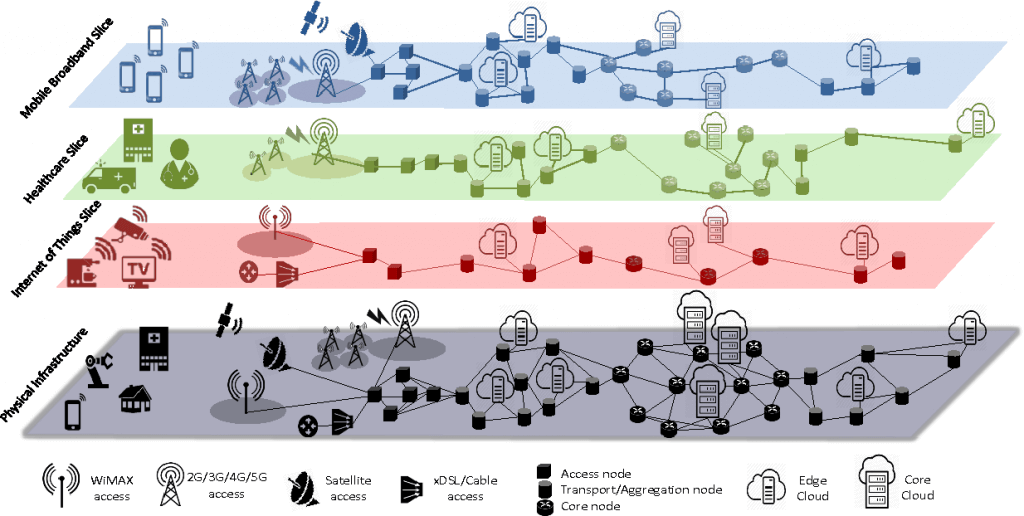
\includegraphics[scale=0.29]{network_slicing_example.png}
        \caption*{\textbf{Fuente}: \url{https://www.onug.net/blog/5g-network-slicing-and-enterprise-networking/}}}
    \end{figure}
\end{frame}

\section{Introducción a SDN}
\begin{frame}{Índice}
    \begin{columns}[t]
        \begin{column}{1.7in}
            \tableofcontents[currentsection, hideallsubsections, sections={1-4}]
        \end{column}
        \begin{column}{1.7in}
            \tableofcontents[currentsection, hideallsubsections, sections={5-7}]
        \end{column}
    \end{columns}
\end{frame}

\begin{frame}{Introducción a SDN}
   \begin{block}{¿Qué es una red SDN?}
        En esencia, el concepto de SDN consiste en la separación entre el plano de control y el plano de datos.
   \end{block}
   \vspace{10pt}
   Analogía con \alert{\textit{Cloud Computing}}.
\end{frame}

\begin{frame}{Introducción a SDN}
    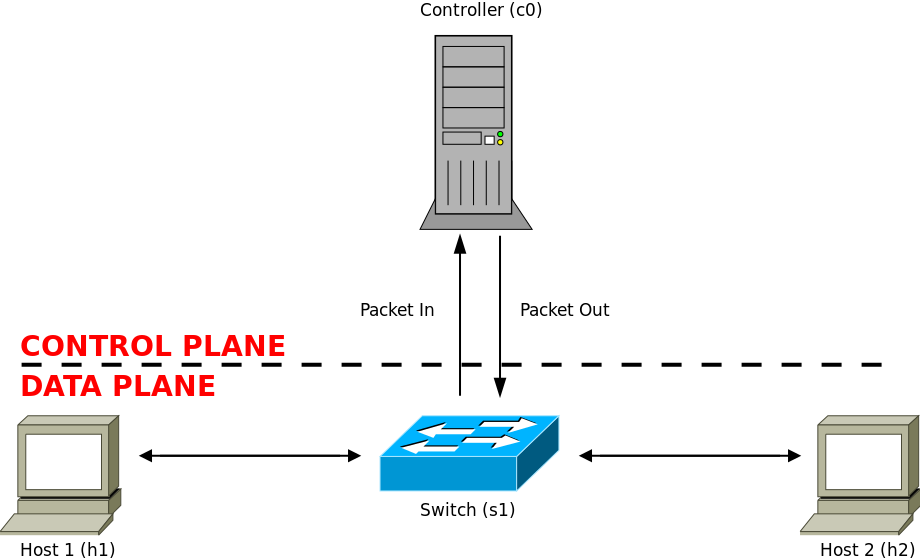
\includegraphics[scale=0.33]{SDN.png}
\end{frame}

\begin{frame}{Introducción a SDN}
    Ventajas de una red SDN frente a una tradicional.\vspace{10pt}
    \begin{itemize}
        \item Flexibilidad y adaptabilidad.
        \item Visión general de la red.
        \item Monitorización.
        \item \textit{Hardware} homogéneo.
        \item Mantenimiento y configuración.
    \end{itemize}
\end{frame}

\section{Descripción de OpenFlow}
\begin{frame}{Índice}
    \begin{columns}[t]
        \begin{column}{1.7in}
            \tableofcontents[currentsection, hideallsubsections, sections={1-4}]
        \end{column}
        \begin{column}{1.7in}
            \tableofcontents[currentsection, hideallsubsections, sections={5-7}]
        \end{column}
    \end{columns}
\end{frame}

\begin{frame}{OpenFlow}
   OpenFlow es el protocolo de comunicación \textit{southbound} más utilizado en redes SDN. \vspace{10pt}
   \begin{block}{\textit{Comunicación southbound}}
        Es la comunicación entre los \textit{forwarding devices} y el controlador o controladores.
   \end{block}\vspace{10pt}

    Los tipos de paquetes más importantes son:
    \begin{itemize}
        \item \textit{Packet\_In}.
        \item \textit{Packet\_Out}.
        \item \textit{FlowMod}.
    \end{itemize}
\end{frame}

\begin{frame}{OpenFlow}
    \centering
    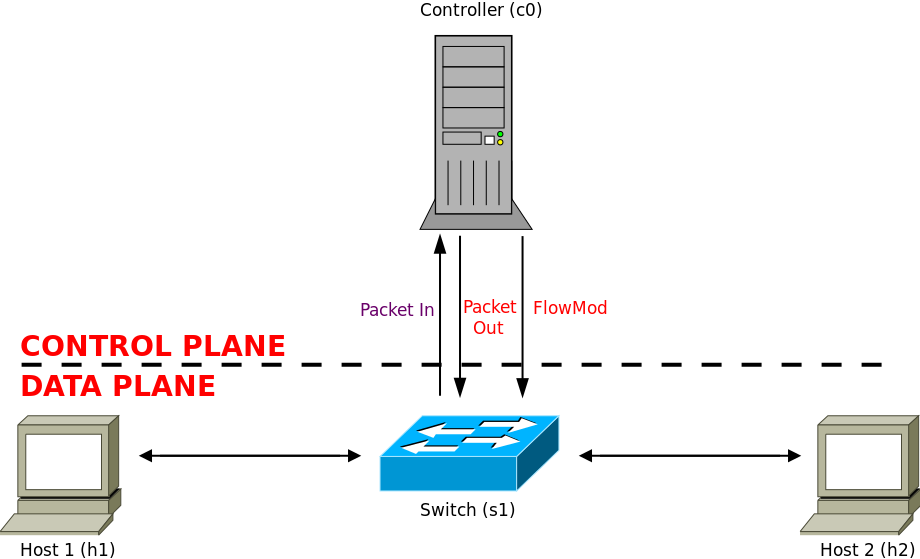
\includegraphics[scale=0.33]{SDN_flowmod.png}
\end{frame}

\begin{frame}[t]{OpenFlow}
    Estructura de una regla de flujo (\textit{flow}) OpenFlow.\vspace{30pt}
    \begin{columns}[t]
    \column{1.9in}
    \textbf{Matching Fields}\\
    Dirección IP destino \\
    Dirección IP origen\\
    Protocolo de Transporte\\
    Puerto TCP destino\\
    Puerto TCP origen\\
    \column{1.9in}
    \textbf{Action}\\
    Enviar por puerto X\\
    Descartar\\
    Packet\_In\\
    Inundar\\
    \end{columns}

    \vspace{40pt}
    \begin{overlayarea}{\textwidth}{2cm}
    \only<2>{sudo ovs-ofctl add-flow s1 nw\_dst=10.0.0.1,actions=output:2}
    \only<3>{sudo ovs-ofctl add-flow \alert{s1} nw\_dst=10.0.0.1,actions=output:2}
    \only<4>{sudo ovs-ofctl add-flow s1 \alert{nw\_dst=10.0.0.1},actions=output:2}
    \only<5>{sudo ovs-ofctl add-flow s1 nw\_dst=10.0.0.1,\alert{actions=output:2}}
    \end{overlayarea}
\end{frame}

\section{Hipervisor OpenFlow}
\subsection{Introducción}
\begin{frame}{Índice}
    \begin{columns}[t]
        \begin{column}{1.7in}
            \tableofcontents[currentsection, subsectionstyle=show/shaded/hide, sections={1-4}]
        \end{column}
        \begin{column}{1.7in}
            \tableofcontents[currentsection, subsectionstyle=show/shaded/hide, sections={5-7}]
        \end{column}
    \end{columns}
\end{frame}

\begin{frame}{Hipervisor OpenFlow}
    \begin{itemize}
        \item Tipo especial de controlador.
        \item Situado entre los \textit{switches} OpenFlow y los controladores.
        \item Intercepta mensajes OpenFlow y los distribuye acorde a su configuración.
        \item Clave para \textit{network slicing}. \textit{Slices}. Múltiples controladores.
        \item Configuración análoga a reglas OpenFlow.
        \item Hipervisor \textit{open source}: \textbf{FlowVisor}.
    \end{itemize}
\end{frame}

\begin{frame}{Hipervisor OpenFlow}\vspace{10pt}
    \centering
    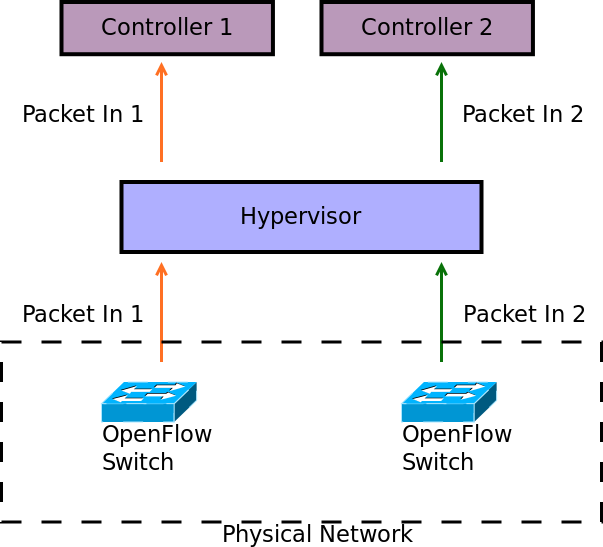
\includegraphics[scale=0.39]{hypervisor.png}
\end{frame}

\subsection{Sintaxis}
\begin{frame}{Índice}
    \begin{columns}[t]
        \begin{column}{1.7in}
            \tableofcontents[currentsection, subsectionstyle=show/shaded/hide, sections={1-4}]
        \end{column}
        \begin{column}{1.7in}
            \tableofcontents[currentsection, subsectionstyle=show/shaded/hide, sections={5-7}]
        \end{column}
    \end{columns}
\end{frame}

\begin{frame}{Hipervisor OpenFlow. FlowVisor Sintaxis}\vspace{25pt}
   \begin{overlayarea}{\textwidth}{6cm}
   Regla ejemplo con la sintaxis usada por FlowVisor. Análogo a las reglas OpenFlow.\vspace{15pt}\\
   \only<1> {fvctl -n add-flowspace example 1 200 in\_port=2 LoRa=6}
   \only<2> {\alert{fvctl -n add-flowspace} example 1 200 in\_port=2 LoRa=6\\[20pt]
            \centering \large \textbf{\textcolor{magenta}{Comando para añadir un flowspace}}}
   \only<3> {fvctl -n add-flowspace \alert{example} 1 200 in\_port=2 LoRa=6\\[20pt]
            \centering \large \textbf{\textcolor{magenta}{Nombre del \textit{flowspace}}}}
   \only<4> {fvctl -n add-flowspace example \alert{1} 200 in\_port=2 LoRa=6\\[20pt]
            \centering \large \textbf{\textcolor{magenta}{Identificador del \textit{switch} (DPID) }}}
   \only<5> {fvctl -n add-flowspace example 1 \alert{200} in\_port=2 LoRa=6\\[20pt]
            \centering \large \textbf{\textcolor{magenta}{Prioridad de la regla}}}
   \only<6> {fvctl -n add-flowspace example 1 200 \alert{in\_port=2} LoRa=6\\[20pt]
            \centering \large \textbf{\textcolor{magenta}{Campo que analizar el paquete}}}
   \only<7> {fvctl -n add-flowspace example 1 200 in\_port=2 \alert{LoRa}=6\\[20pt]
            \centering \large \textbf{\textcolor{magenta}{\textit{Slice} al que asignar el paquete}}}
   \only<8> {fvctl -n add-flowspace example 1 200 in\_port=2 LoRa\alert{=6}\\[20pt]
            \centering \large \textbf{\textcolor{magenta}{Permisos del slice}}}
    \end{overlayarea}
\end{frame}

\subsection{Ventajas}
\begin{frame}{Índice}
    \begin{columns}[t]
        \begin{column}{1.7in}
            \tableofcontents[currentsection, subsectionstyle=show/shaded/hide, sections={1-4}]
        \end{column}
        \begin{column}{1.7in}
            \tableofcontents[currentsection, subsectionstyle=show/shaded/hide, sections={5-7}]
        \end{column}
    \end{columns}
\end{frame}

\begin{frame}{Network Slicing. Ventajas y Aplicaciones}
    \textbf{Ventajas}
    \begin{itemize}
        \item Simplificación de la lógica de los controladores.
        \item Mantenimiento.
        \item Adaptabilidad.
        \item Aislamiento entre \textit{slices}.
    \end{itemize}
    \vspace{20pt}
    \textbf{Aplicaciones}
    \begin{itemize}
        \item Ingeniería de tráfico.
        \item Multiplexación de servicios en la misma red física.
        \item Uso de una red de producción como escenario de pruebas.
    \end{itemize}
\end{frame}

\section{Implementación}
\subsection{Virtualización}
\begin{frame}{Índice}
    \begin{columns}[t]
        \begin{column}{1.7in}
            \tableofcontents[currentsection, subsectionstyle=show/shaded/hide, sections={1-4}]
        \end{column}
        \begin{column}{1.7in}
            \tableofcontents[currentsection, subsectionstyle=show/shaded/hide, sections={5-7}]
        \end{column}
    \end{columns}
\end{frame}

\begin{frame}{Virtualización}
   No disponemos de \textit{switches} OpenFlow para montar una red SDN. Tenemos que recurrir a emulación.\vspace{10pt}
   \begin{itemize}
       \item Open vSwitch.
       \item Mininet.
       \item Iperf.
   \end{itemize}\vspace{10pt}

   \onslide<2> Como controlador OpenFlow usaremos \textbf{POX}.
\end{frame}

\begin{frame}{Virtualización. Topología}
    \centering
    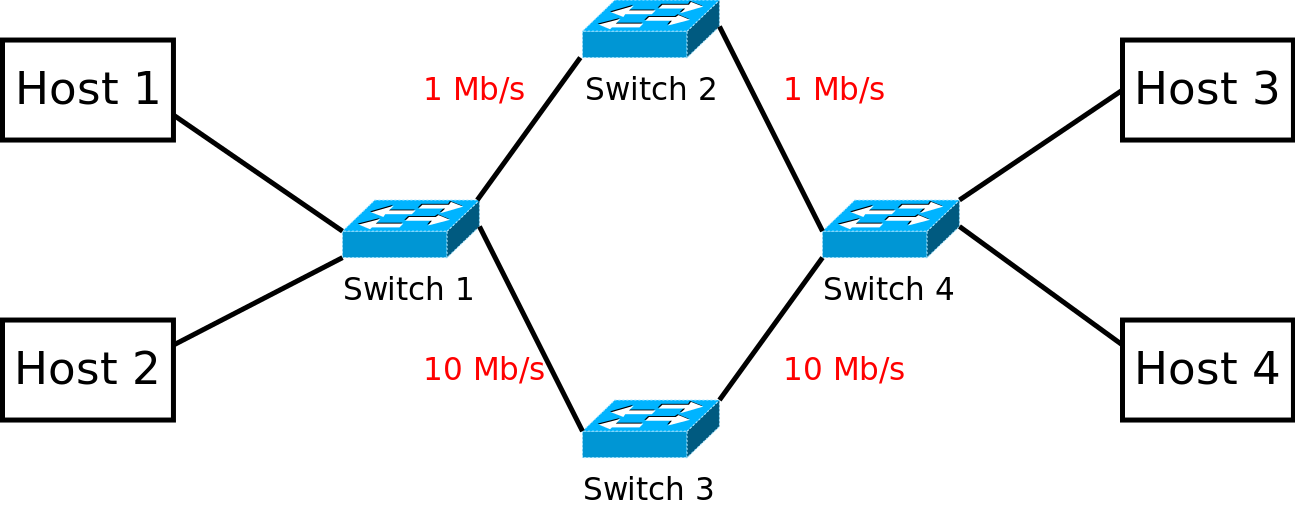
\includegraphics[scale=0.23]{mininet_topology.png}
\end{frame}


\subsection{TCP Port Slicing}
\begin{frame}{Índice}
    \begin{columns}[t]
        \begin{column}{1.7in}
            \tableofcontents[currentsection, subsectionstyle=show/shaded/hide, sections={1-4}]
        \end{column}
        \begin{column}{1.7in}
            \tableofcontents[currentsection, subsectionstyle=show/shaded/hide, sections={5-7}]
        \end{column}
    \end{columns}
\end{frame}

\begin{frame}{TCP Port Slicing}
    \centering
    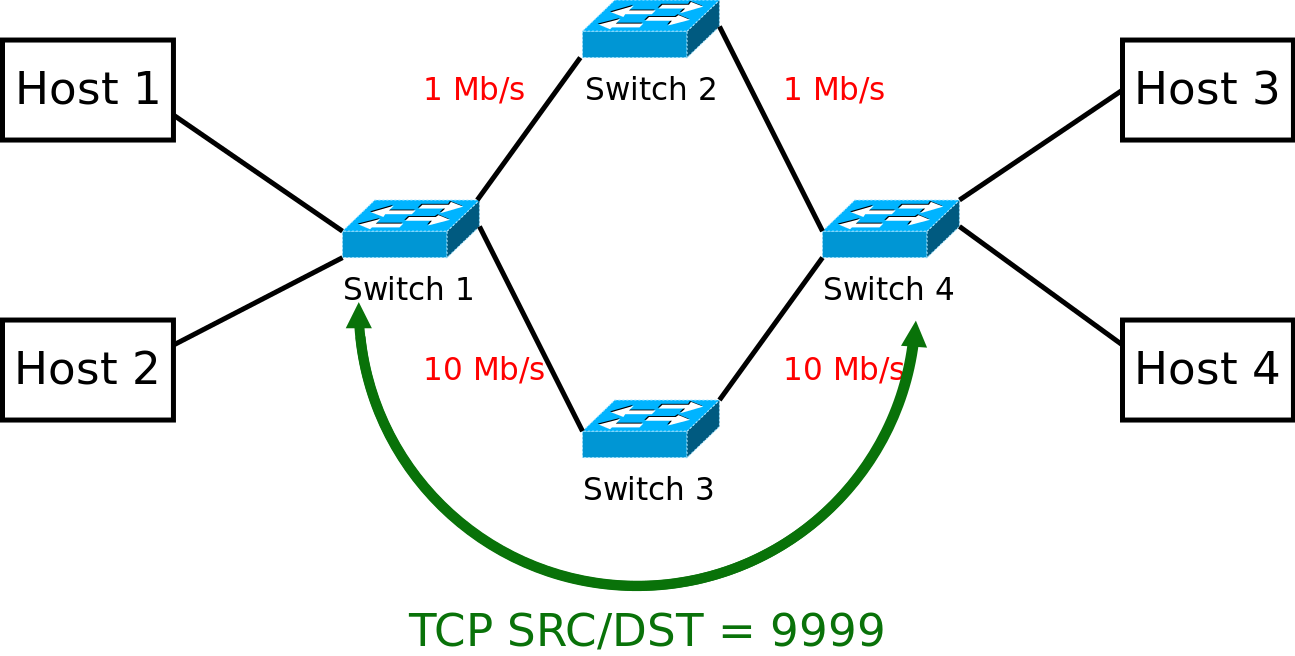
\includegraphics[scale=0.23]{mininet_topology_port_slicing.png}
\end{frame}

\subsection{Demo TCP Port Slicing}
\begin{frame}{Índice}
    \begin{columns}[t]
        \begin{column}{1.7in}
            \tableofcontents[currentsection, subsectionstyle=show/shaded/hide, sections={1-4}]
        \end{column}
        \begin{column}{1.7in}
            \tableofcontents[currentsection, subsectionstyle=show/shaded/hide, sections={5-7}]
        \end{column}
    \end{columns}
\end{frame}

\subsection{IP Address Slicing}
\begin{frame}{Índice}
    \begin{columns}[t]
        \begin{column}{1.7in}
            \tableofcontents[currentsection, subsectionstyle=show/shaded/hide, sections={1-4}]
        \end{column}
        \begin{column}{1.7in}
            \tableofcontents[currentsection, subsectionstyle=show/shaded/hide, sections={5-7}]
        \end{column}
    \end{columns}
\end{frame}

\begin{frame}{IP Address Slicing}
    \centering
    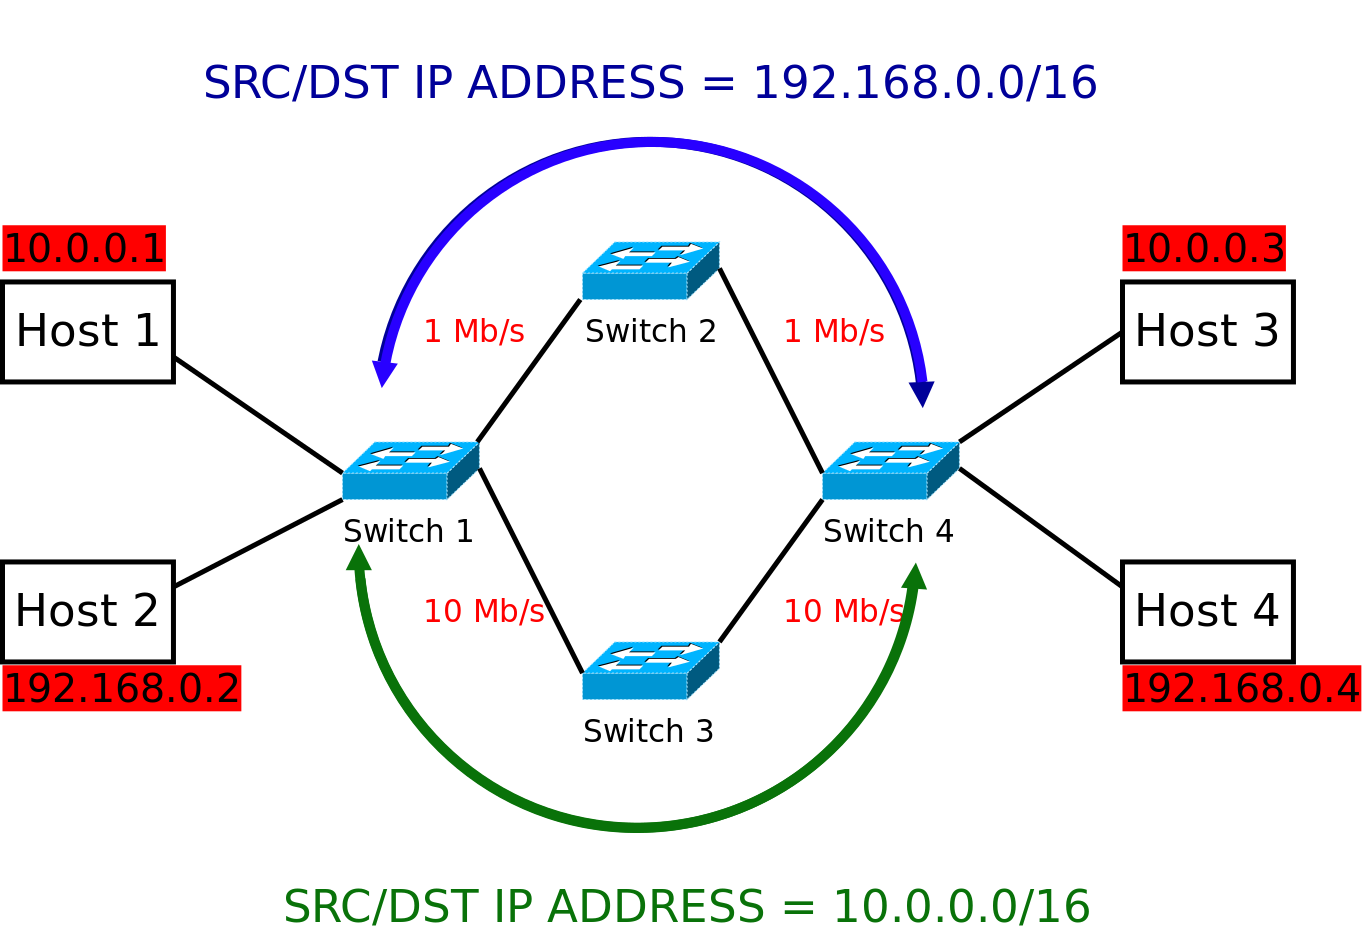
\includegraphics[scale=0.22]{mininet_topology_IP_slicing.png}
\end{frame}

\begin{frame}{IP Address Slicing}
    \centering
    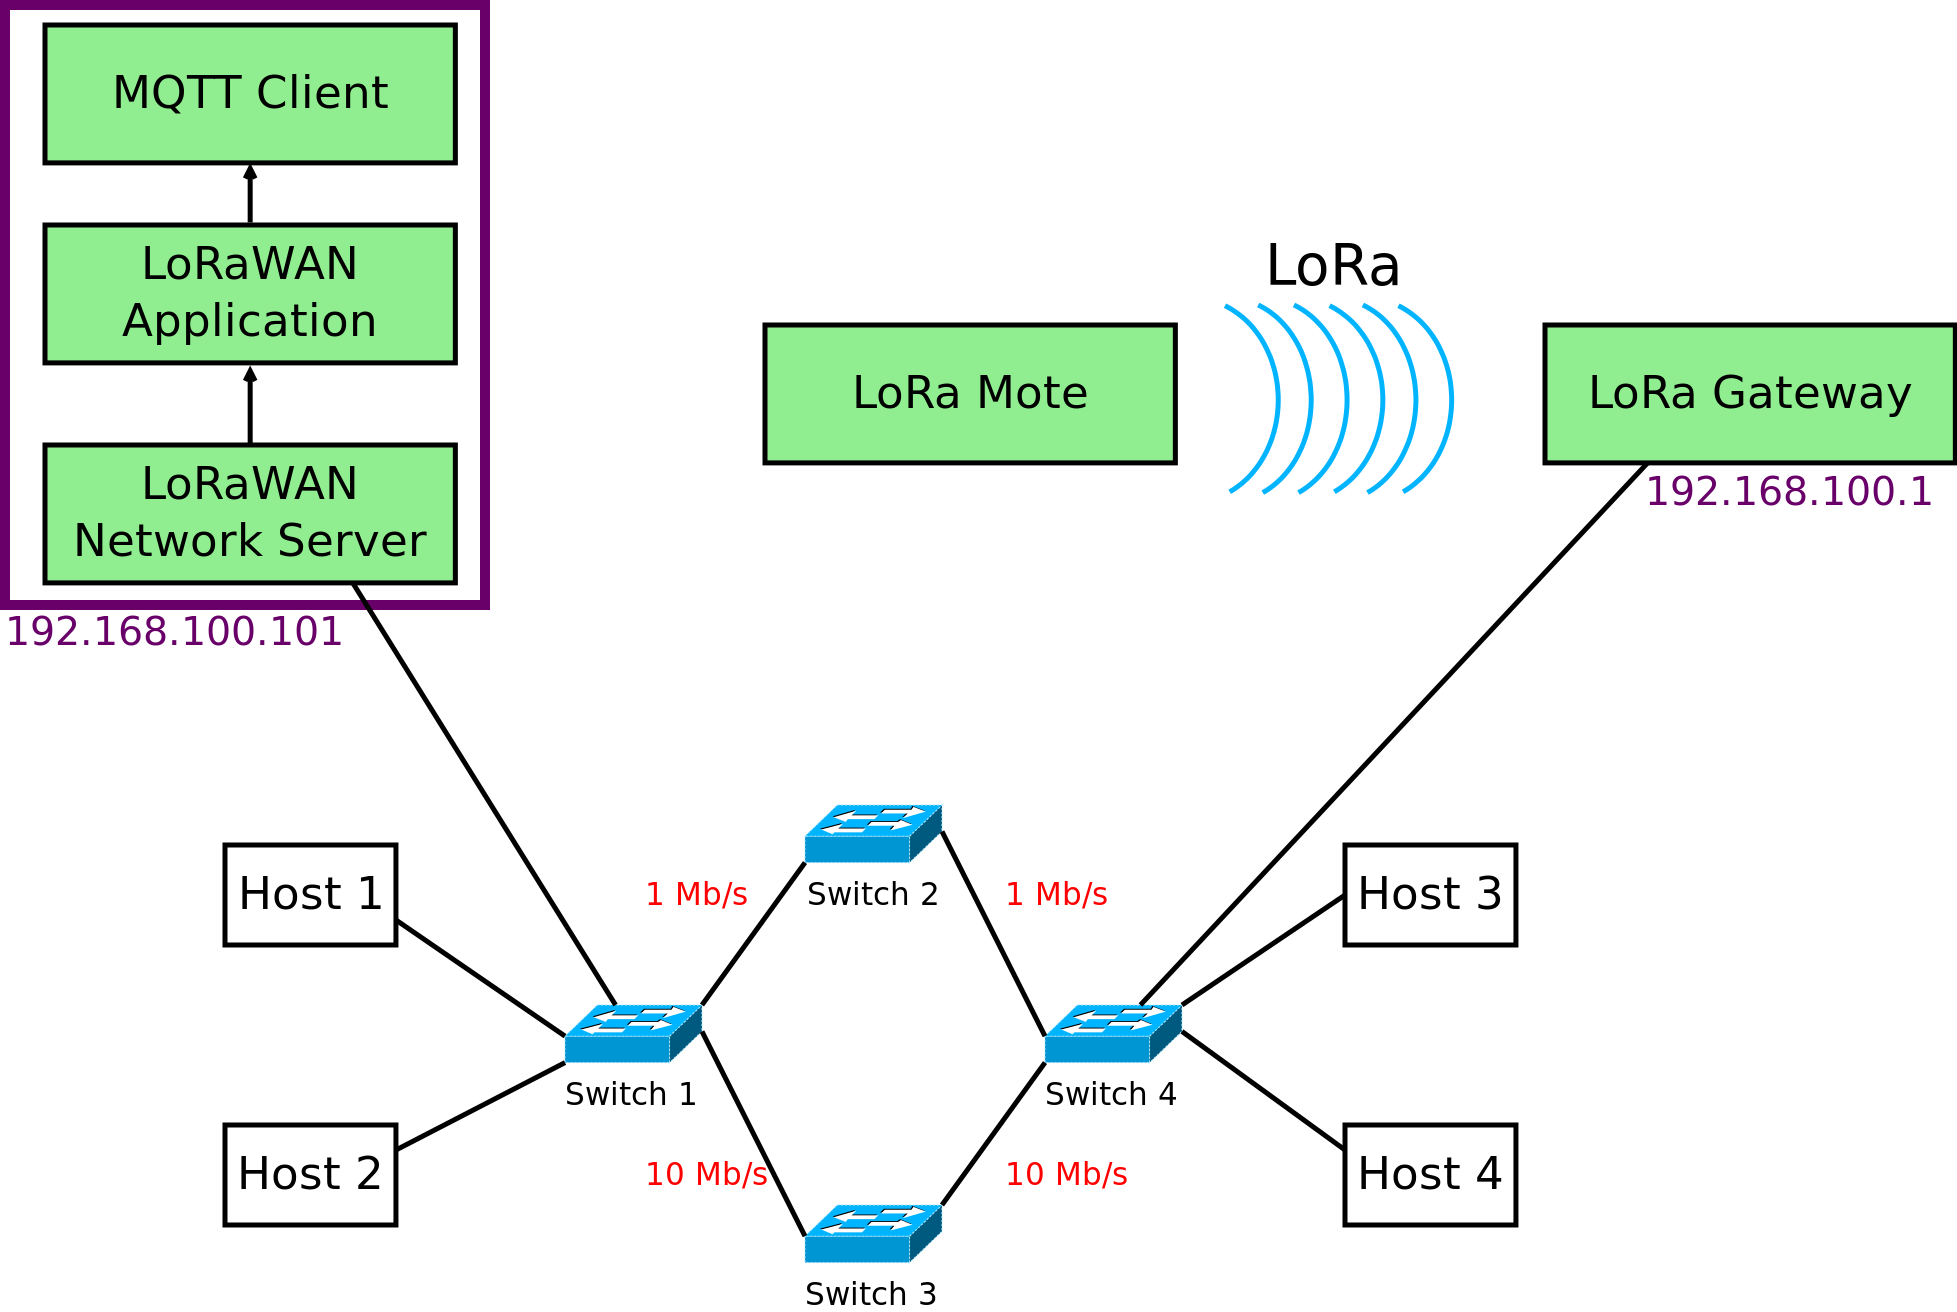
\includegraphics[scale=0.155]{mininet_topology_LoRa.png}
\end{frame}

\begin{frame}{IP Address Slicing}
    \centering
    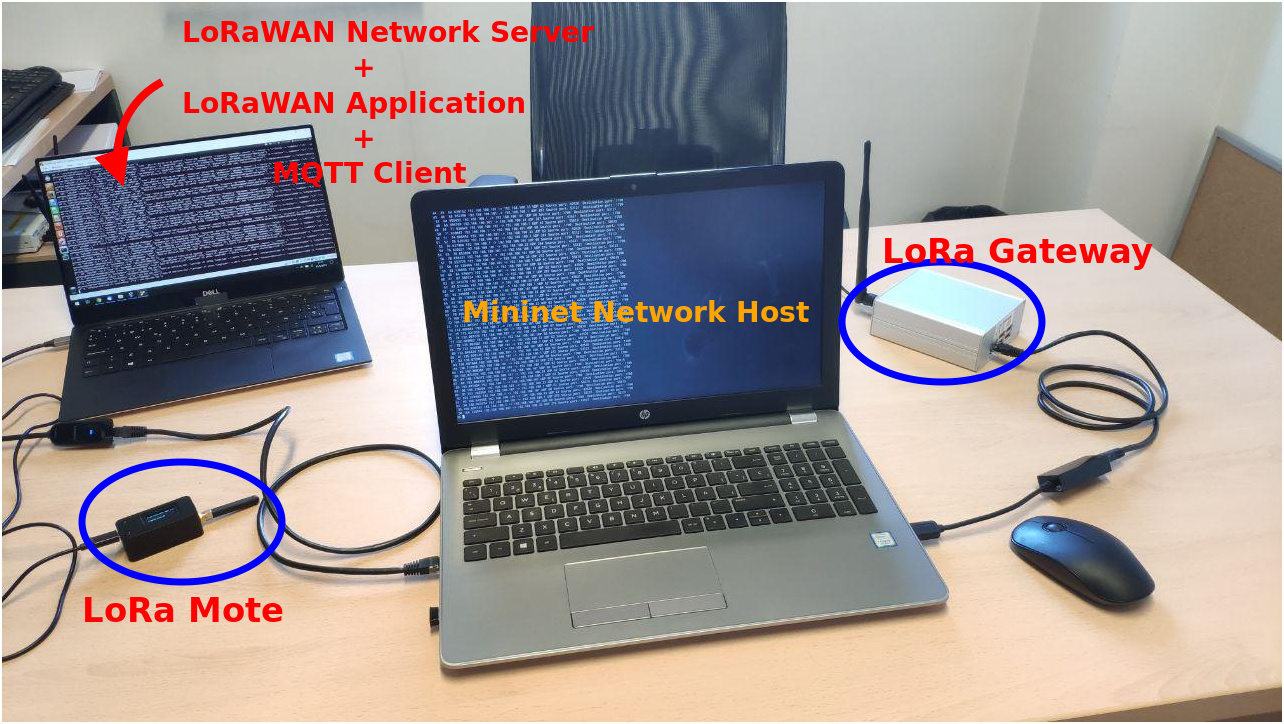
\includegraphics[scale=0.23]{lora_setup.png}
\end{frame}

\subsection{Demo IP Address Slicing}
\begin{frame}{Índice}
    \begin{columns}[t]
        \begin{column}{1.7in}
            \tableofcontents[currentsection, subsectionstyle=show/shaded/hide, sections={1-4}]
        \end{column}
        \begin{column}{1.7in}
            \tableofcontents[currentsection, subsectionstyle=show/shaded/hide, sections={5-7}]
        \end{column}
    \end{columns}
\end{frame}

\section{Conclusiones}
\begin{frame}{Índice}
    \begin{columns}[t]
        \begin{column}{1.7in}
            \tableofcontents[currentsection, hideallsubsections, sections={1-4}]
        \end{column}
        \begin{column}{1.7in}
            \tableofcontents[currentsection, hideallsubsections, sections={5-7}]
        \end{column}
    \end{columns}
\end{frame}

\begin{frame}{Conclusiones}
    \textbf{¿Hemos cumplido con los objetivos?}\vspace{10pt}
    \begin{itemize}
        \item Hemos entendido las limitaciones de redes tradicionales.
        \item Familiarización con redes SDN y \textit{network slicing}.
        \item Particionado de red de dos formas diferentes.
    \end{itemize}\vspace{20pt}

    \onslide<2>{\textbf{Respecto al \textit{network slicing}}.\vspace{10pt}
    \begin{itemize}
        \item Solución al tráfico heterogéneo.
        \item Alternativa a \textit{QoS}.
        \item Simplifica la configuración del controlador o controladores.
        \item Aislamiento entre secciones de la misma red.
    \end{itemize}}
\end{frame}

\end{document}
